
\documentclass{article}
\usepackage{booktabs} % For \toprule, \midrule, and \bottomrule
\usepackage{multirow} % For \multirow
\usepackage{geometry} % For adjusting page dimensions (optional)
\geometry{a4paper, margin=1in} % Adjust margins as needed

\usepackage{pgfplots}
\pgfplotsset{compat=1.18}

\usepackage{siunitx} % For scientific notation
\sisetup{output-exponent-marker=\text{e}} % Optional: to use 'e' notation

\begin{document}

% Your table code here
\begin{table}[htbp]
\centering
\begin{tabular}{@{}ccccccc@{}}
\toprule
\multirow{2}{*}{Qubits} & \multicolumn{3}{c}{TOWER\_CHEBYSHEV} & \multicolumn{3}{c}{FNN\_BASIS} \\
\cmidrule(lr){2-4} \cmidrule(l){5-7}
& Loss & $L_2$ & $L_\infty$ & Loss & $L_2$ & $L_\infty$ \\
\midrule
2 & \num{3.68e1} & \num{3.23e-2} & \num{3.17e-1} & \num{6.76e-2} & \num{3.03e-5} & \num{4.00e-2} \\
4 & \num{5.49e0} & \num{2.28e-3} & \num{1.23e-1} & \num{7.87e-3} & \num{3.43e-6} & \num{2.45e-2} \\
6 & \num{8.87e-1} & \num{2.05e-4} & \num{3.31e-2} & \num{4.48e-3} & \num{4.60e-6} & \num{2.08e-2} \\
8 & \num{3.49e-1} & \num{1.07e-4} & \num{2.65e-2} & \num{1.89e-3} & \num{4.19e-6} & \num{1.23e-2} \\
\bottomrule
\end{tabular}
\caption{Comparison of TOWER\_CHEBYSHEV and FNN\_BASIS metrics for different numbers of qubits}
\label{tab:quantum-metrics}
\end{table}


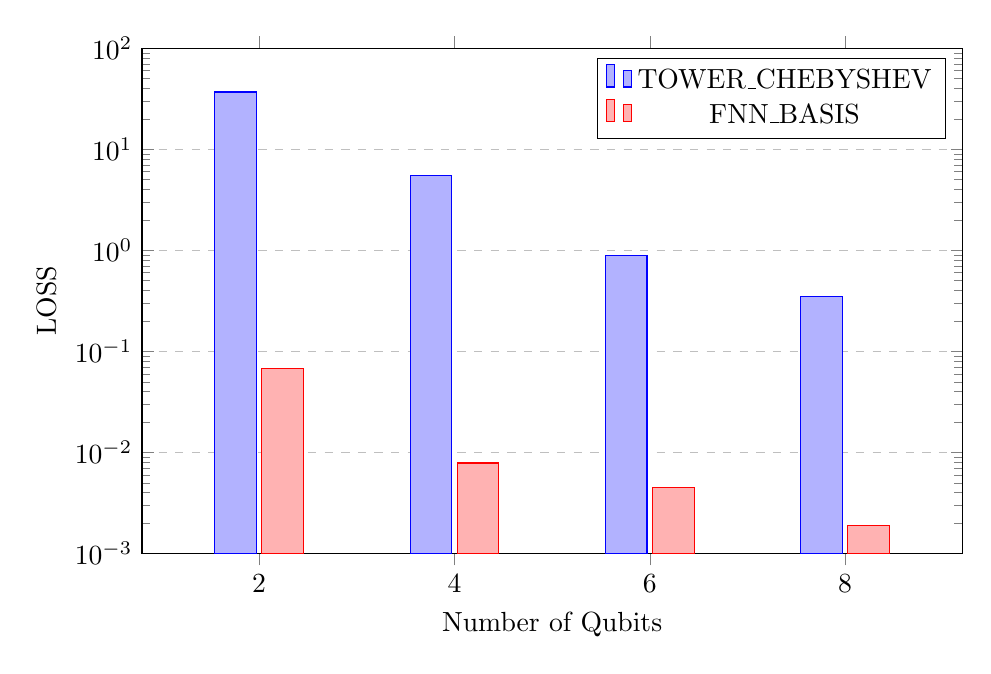
\begin{tikzpicture}
\begin{axis}[
    ybar,
    bar width=15pt,
    width=12cm,
    height=8cm,
    % legend style={at={(0.5,-0.15)}, anchor= intern north, legend columns=-1},
    ylabel={LOSS},
    xlabel={Number of Qubits},
    symbolic x coords={2,4,6,8},
    xtick=data,
    ymode=log,
    log origin=infty,
    ymin=1e-3,
    ymax=100,
    ymajorgrids=true,
    grid style=dashed,
    enlarge x limits=0.2,
    point meta=rawy,
]

\addplot coordinates {(2,36.8) (4,5.49) (6,0.887) (8,0.349)};
\addplot coordinates {(2,0.0676) (4,0.00787) (6,0.00448) (8,0.00189)};

\legend{TOWER\_CHEBYSHEV, FNN\_BASIS}

\end{axis}
\end{tikzpicture}

\end{document}